
\documentclass[12pt,onecolumn]{IEEEtran}
%packages
\usepackage{cite}
\usepackage{gensymb}
\usepackage{amssymb,amsmath}
\usepackage{textcomp}
\usepackage{csquotes}
\usepackage{graphicx}
\usepackage{blindtext, graphicx}
\graphicspath{ {imgs/} }

\usepackage{dblfloatfix} 
% *** GRAPHICS RELATED PACKAGES ***
%
\ifCLASSINFOpdf
  % \usepackage[pdftex]{graphicx}
  % declare the path(s) where your graphic files are
  % \graphicspath{{../pdf/}{../jpeg/}}
  % and their extensions so you won't have to specify these with
  % every instance of \includegraphics
  % \DeclareGraphicsExtensions{.pdf,.jpeg,.png}
\else
  % or other class option (dvipsone, dvipdf, if not using dvips). graphicx
  % will default to the driver specified in the system graphics.cfg if no
  % driver is specified.
  % \usepackage[dvips]{graphicx}
  % declare the path(s) where your graphic files are
  % \graphicspath{{../eps/}}
  % and their extensions so you won't have to specify these with
  % every instance of \includegraphics
  % \DeclareGraphicsExtensions{.eps}
\fi

\hyphenation{op-tical net-works semi-conduc-tor}


\begin{document}
\title{Review on \\ Towards 1 Gbps/UE in Cellular Systems: Understanding Ultra-Dense Small Cell Deployments}
\author{\IEEEauthorblockN{Sai Narsi Reddy Donthi Reddy}\\
\IEEEauthorblockA{School of Computing and Engineering\\
University of Missouri -  Kansas City\\
Email: sdhy7@mail.umkc.edu\\
UMKC ID: 16186610}}
\maketitle



\section{Introduction}
\label{sec:intro}

-- Intro --

\section{Paper Outline}
\label{sec:PO}

 \renewcommand{\theenumi}{\Roman{enumi}}
 \begin{enumerate}
   \item Abstract
   \item Index Terms
   \item Introduction
   \item Small Cells in HetNets
   \item Why Are Today's Small Cells Not Practical to Meet Future Capacity Demands?
   \item System Model
   \item Network Densification
   \begin{enumerate}
     \item Idel Mode Capability and the 1 UE per cell concept
     \item Transmit Power and UE SINR Distribution
     \begin{enumerate}
     \item Transmit Power
     \item UE SINR Distribution
     \end{enumerate}
     \item Transition From the Interference-Limited Regime to the Noise-limited Regime
     \end{enumerate}
   \item Higher Frequency Bands
   \item Multi-antenna Techniques and Beamforming
   \item Scheduling
   \item Energy-Efficiency
   \item What is Different in Ultra-Dense Small Cell Deployments
   \item Challenges in Ultra-Dense Small Cell Deployments
   \item Conclusion
   \item Appendix
   \item References
 \end{enumerate}

\section{The Problem}
\label{sec:TP}
It is estimated that by 2020 at least 100 folds network capacity should be increase to meet the oncoming demand. Currently, vendors and operators are implementing different technologies to improve the network capacity. All the existing tools can be classified into three categories as show in figure - \ref{fig:NWCP}. First, increasing spatial reuse by network densification  which is been done by increasing type-2 small cells in a type-1 macro cells (HetNet architecture). Second, By exploring higher spectrum frequencies which gives higher bandwidth per cell. And lastly, more spectral efficiency by using multi-antenna system, dynamic TDD etc,. However, these improvements are not enough to meet the future demand. Due to large difference in transmission power between macro cell and co-channel small cell (Type-2 cells), UE's tend to connect to macro cell base station (BS) rather than high speed small cell. When it comes to spectrum frequency bands, the current generation still uses spectrum frequencies in range of 1-2Ghz. These, spectrum frequency ranges have very low bandwidth and results in lower data rates.

\begin{figure}[ht]
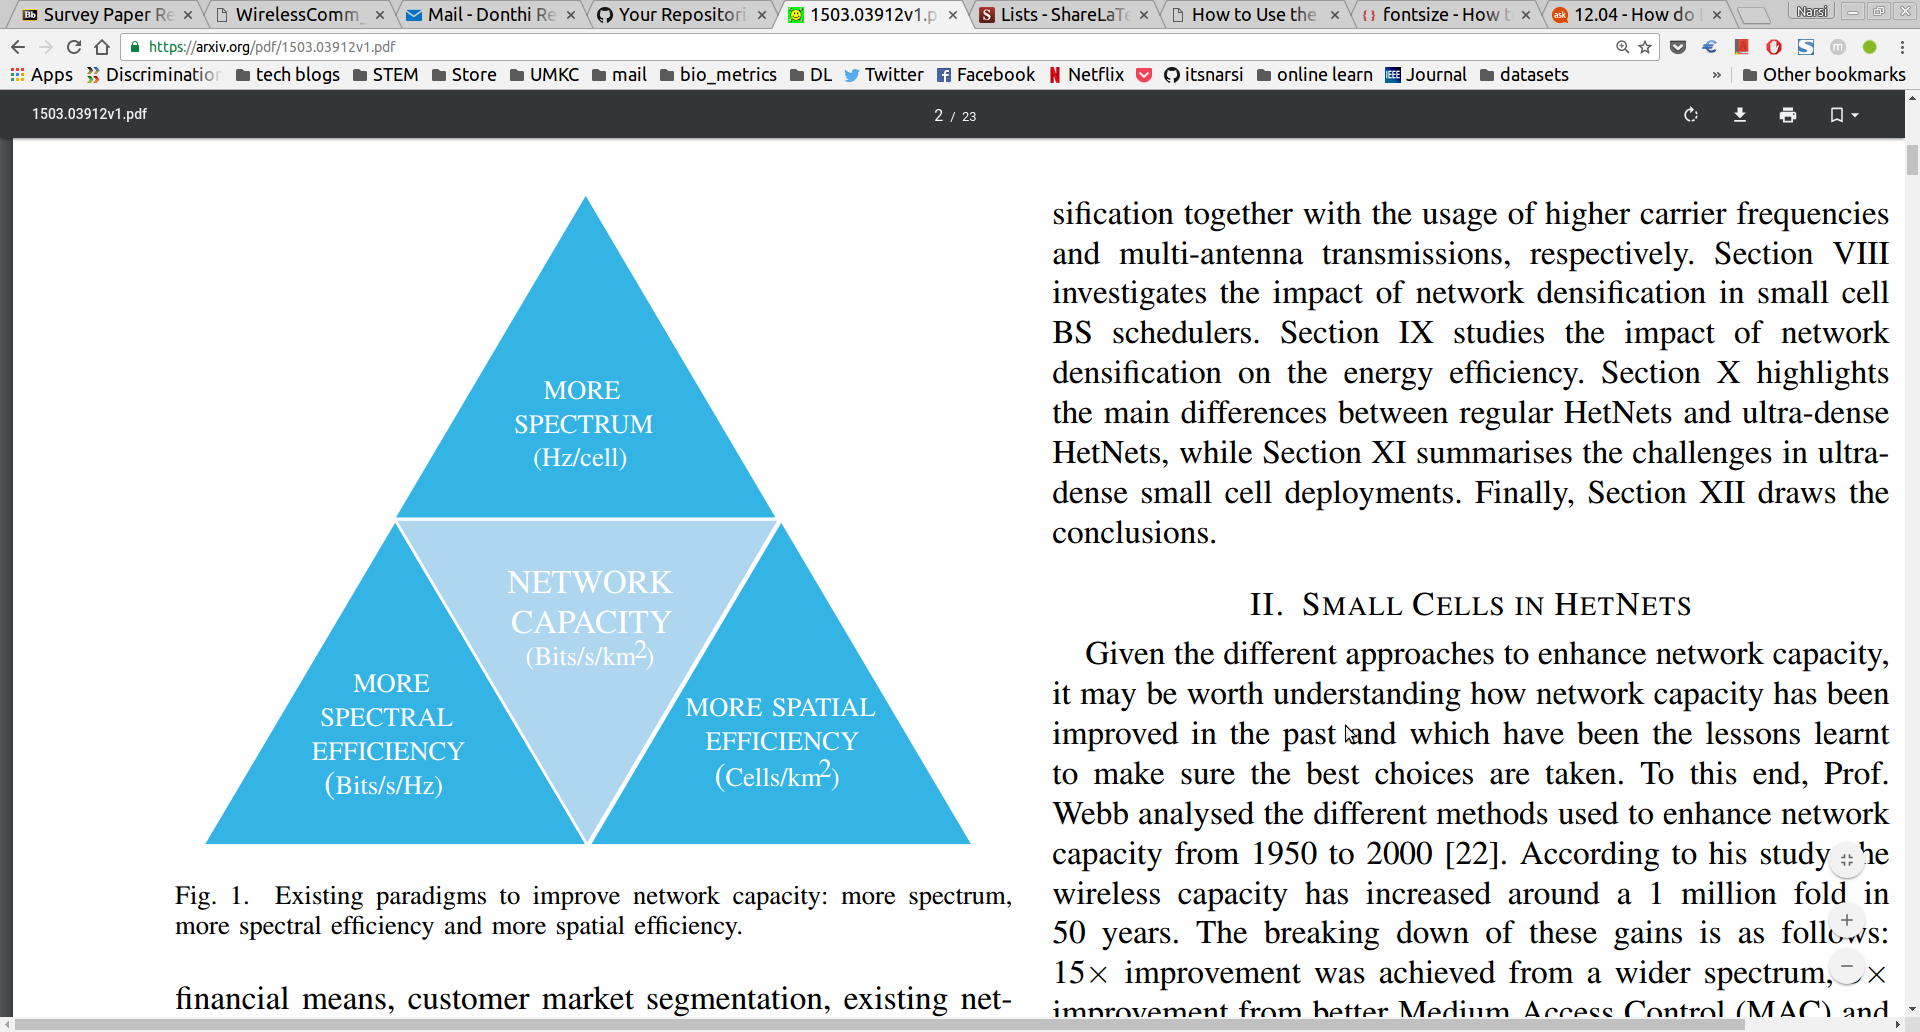
\includegraphics[scale=0.3]{nwcp_class}
\centering
\caption{Three categories of existing tools to improve Network capacity.}
\label{fig:NWCP}
\end{figure}

It is important to address these issue as in coming years with the increase in number of UE's and necessary high speed data, the current generation wireless technologies are not capable of handling theses trends. These problems can be overcome by using better network densification techniques, higher frequency spectrum and spectral efficiency techniques which are discuss in section - \ref{sec:TC}.


\section{The Application}
\label{sec:TA}

In the early days of wireless communication systems, voice service is the most demanding service with requirements of tens of Kbps per user equipment (UE). However, these days video steaming is the service with high demand requiring tens of Mbps per UE ~\cite{stream_vid}. 
In future, with increase internet of things (IOT) applications such as home automation, monitoring, infrastructure management and autonomous cars etc., the number of UE count increase drastically. 
With the rapid growth in virtual reality (VR) and augmented reality (AR) the requirement for low latency data increase in the gaming applications. 
The streming media services are moving towards higher resolution technologies such as 4K and 8K resolutions require very high data rates ~\cite{youtube}.

The above demands can be meet only by increasing network capacity by atleast 100 folds. This can be achieved by applying modern techniques in wireless communications. Some of them are discussed in section - \ref{sec:TC}.

\section{The Categories}  
\label{sec:TC}

\section{The Future}
\label{sec:TF}

\section{What We Learn?}
\label{sec:WWL}

\section{Five Most Important Points}
\label{sec:FMIP}
% Can use something like this to put references on a page
% by themselves when using endfloat and the captionsoff option.
\ifCLASSOPTIONcaptionsoff
  \newpage
\fi

\bibliographystyle{IEEEtran}
\bibliography{biblio}

\end{document}


